\newpage
\section{Sue de Coq}
Die Technik \textit{Sue de Coq} wurde ursprünglich unter dem Namen \textit{Two-Sector Disjoint Subsets} in einem Forum\footnote{\url{http://forum.enjoysudoku.com/two-sector-disjoint-subsets-t2033.html}} vorgestellt. Anderen Benutzern des Forums war dieser Name zu umständlich und sie begannen die Strategie als \textit{Sue de Coq} zu bezeichnen, dem Benutzernamen des Vorstellers.\\
Um die Technik anzuwenden sucht man zuerst zwei oder drei Zellen in einem Block, die in der selben Reihe oder Spalte liegen. Die Vereinigung der Kandidatenlisten muss dabei bei zwei Zellen vier Kandidaten enthalten und bei drei Zellen müssen fünf Kandidaten vorhanden sein. Nun sucht man zusätzlich eine Zelle im selben Block, die ausschließlich zwei Kandidaten der Vereinigung enthält. Eine solche Zelle sucht man auch in der Reihe oder Spalte, in der die ersten Zellen liegen. Die Schnittmenge der Kandidatenlisten der beiden zusätzlichen Zellen muss leer sein. \\
Die Kandidaten aus der zusätzlichen Zelle in der Reihe können nun aus allen unbeteiligten Zellen der Reihe gelöscht werden.  Das gilt ebenfalls für die Kandidaten der zusätzlichen Zelle des Blocks, diese können aus allen unbeteiligten Zellen des Blocks entfernt werden.\\

\begin{figure}[h]
\begin{center}
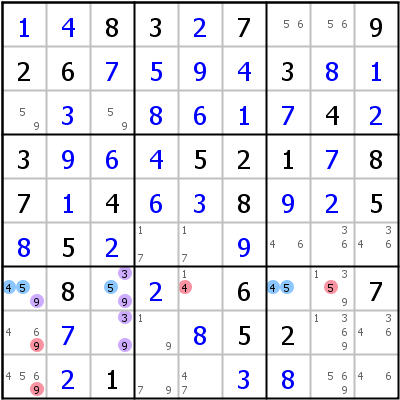
\includegraphics{./img/Sue_de_Coq.png}
\caption{Sue de Coq}
\end{center}
\end{figure}

In Abbildung \textbf{3.16} sieht man einen \textit{Sue de Coq} mit den zwei Basiszellen z7s1 und z7s3. Diese liegen im Block 7 in der selben Zeile. Die Vereinigung der Kandidaten enthält die Ziffern 3, 4, 5 und 9. Die zusätzliche Zelle in der Zeile ist z7s7. Sie enthält die Kandidaten 4 und 5 die Teilmenge der vorherigen Vereinigung ist. Die zusätzliche Zelle im Block 7 ist z8s3. Diese enthält die Kandidaten 3 und 9, die ebenfalls Teilmenge der Vereinigung ist. der Schnitt der Kandidatenlisten der zusätzlichen Zellen ist leer. Damit sind alle Bedingungen für den \textit{Sue de Coq} erfüllt und die rot markierten Kandidaten können gelöscht werden.